% Generated LaTeX file for compound CID: 101258
\documentclass[tikz]{standalone}
\definecolor{274A4A}{HTML}{274A4A}
\definecolor{2AD52A}{HTML}{2AD52A}
\definecolor{D5D500}{HTML}{D5D500}
\definecolor{FF0000}{HTML}{FF0000}
\begin{document}
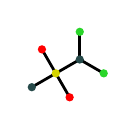
\begin{tikzpicture}[x=1pt,y=1pt]
  \draw[line width=1pt] (45.98,-3.17) -- (37.32,1.83);
  \draw[line width=1pt] (37.32,11.83) -- (37.32,1.83);
  \draw[line width=1pt] (28.66,-3.17) -- (23.66,5.49);
  \draw[line width=1pt] (28.66,-3.17) -- (33.66,-11.83);
  \draw[line width=1pt] (28.66,-3.17) -- (37.32,1.83);
  \draw[line width=1pt] (28.66,-3.17) -- (20.00,-8.17);
  \filldraw[fill=2AD52A, draw=none] (45.98,-3.17) circle (1.5pt);
  \filldraw[fill=2AD52A, draw=none] (37.32,11.83) circle (1.5pt);
  \filldraw[fill=D5D500, draw=none] (28.66,-3.17) circle (1.5pt);
  \filldraw[fill=FF0000, draw=none] (23.66,5.49) circle (1.5pt);
  \filldraw[fill=FF0000, draw=none] (33.66,-11.83) circle (1.5pt);
  \filldraw[fill=274A4A, draw=none] (37.32,1.83) circle (1.5pt);
  \filldraw[fill=274A4A, draw=none] (20.00,-8.17) circle (1.5pt);
\end{tikzpicture}
\end{document}